\documentclass{article}
\usepackage{fancyhdr}
\usepackage{ctex}
\usepackage{listings}
\usepackage{graphicx}
\usepackage[a4paper, body={18cm,22cm}]{geometry}
\usepackage{amsmath,amssymb,amstext,wasysym,enumerate,graphicx}
\usepackage{float,abstract,booktabs,indentfirst,amsmath}
\usepackage{array}
\usepackage{booktabs}
\usepackage{multirow}
\usepackage{url}
\usepackage{diagbox}
\renewcommand\arraystretch{1.4}
\usepackage{indentfirst}
\setlength{\parindent}{2em}
\usepackage{enumitem}
\setmonofont{Consolas}
\usepackage{listings}
\usepackage{xcolor}
\usepackage{makecell}
\setCJKmonofont{黑体}
\lstset{
    % language = C,
    xleftmargin = 3em,xrightmargin = 3em, aboveskip = 1em,
	backgroundcolor = \color{white}, % 背景色
	basicstyle = \small\ttfamily, % 基本样式 + 小号字体
	rulesepcolor= \color{gray}, % 代码块边框颜色
	breaklines = true, % 代码过长则换行
	numbers = left, % 行号在左侧显示
	numberstyle = \small, % 行号字体
    numbersep = -14pt, 
    keywordstyle=\color{purple}\bfseries, % 关键字颜色
    commentstyle =\color{red!50!green!50!blue!60}, % 注释颜色
    stringstyle = \color{red}, % 字符串颜色
    morekeywords={ASSERT, int64_t, uint32_t},
	frame = shadowbox, % 用(带影子效果)方框框住代码块
	showspaces = false, % 不显示空格
	columns = fixed, % 字间距固定
} 
\lstset{
    sensitive=true,
    moreemph={ASSERT, NULL}, emphstyle=\color{red}\bfseries,
    moreemph=[2]{int64_t, uint32_t, tid_t, uint8_t, int16_t, uint16_t, int32_t, size_t}, emphstyle=[2]\color{purple}\bfseries,
    }
%--------------------页眉--------------------%
\pagestyle{fancy}
\fancyhead[L]{}
\fancyhead[R]{}
\fancyhead[C]{华东师范大学软件工程学院实验报告}
\fancyfoot[C]{-\thepage-}
\renewcommand{\headrulewidth}{1.5pt}
%--------------------标题--------------------%
\begin{document}
\begin{center}
  \LARGE{{\textbf{\heiti 华东师范大学软件工程学院实验报告}}}
  \begin{table}[H]
    \centering
    \begin{tabular}{p{2cm}p{4cm}<{\centering}p{1cm}p{2cm}p{4cm}<{\centering}}
      实验课程:    & 计算机网络 & \quad & 年\qquad 级: & 2023级      \\ \cline{2-2} \cline{5-5}
      实验编号:    & Lab 02     & \quad & 实验名称:    & Ethernet
      \\ \cline{2-2} \cline{5-5}
      姓\qquad 名: & 王海生     & \quad & 学\qquad 号: & 10235101559 \\ \cline{2-2} \cline{5-5}
    \end{tabular}
  \end{table}
\end{center}
\rule{\textwidth}{1pt}
%--------------------正文--------------------%
\section{实验目的}
\begin{enumerate}[noitemsep, label={{\arabic*})}]
  \item 学会通过Wireshark获取以太网的帧
  \item 掌握以太网帧的结构
  \item 分析以太网地址范围
  \item 分析以太网的广播帧
\end{enumerate}
\section{实验内容与实验步骤}
\subsection{实验内容}


\subsubsection{获取以太网的帧}
在命令行中使用\texttt{ping}命令发起\texttt{ICMP}请求,然后使用\texttt{Wireshark}捕获\texttt{以太网}数据包。

\subsubsection{分析以太网的帧}

分析\texttt{以太网}的帧,画出帧结构。

\subsubsection{分析以太网的地址范围}

分析\texttt{以太网}的地址范围,画出图示关系图。

\subsubsection{分析以太网的广播帧}

启动Wireshark,在菜单栏的捕获\(\to \)选项中进行设置,选择已连接的以太网,设置捕获过滤器为\texttt{ether multicast},捕获\texttt{以太网}的广播帧。

分析\texttt{以太网}的广播帧,回答以下问题:

\begin{enumerate}[noitemsep]
  \item 以太网广播帧的地址是什么,以标准的形式写在Wireshark上显示?
  \item 哪几个比特位的以太网地址是用来确定是单播或多播/广播?
\end{enumerate}

\subsubsection{问题讨论}

\begin{enumerate}[noitemsep]
  \item 与DIX以太网报头相比,IEEE 802.3和LLC组合报头有多长?
  您可以使用Wireshark解决此问题。 请注意,Trailer / Padding和Checksum可能显示为标头的一部分,但它们位于帧的末尾。
  
  \item 接收方计算机如何知道该帧是DIX以太网还是IEEE 802.3? 提示:您可能需要同时使用Wireshark查看数据包示例并查找相关文献。
  
  \item 如果IEEE 802.3没有类型字段,那么如何确定下一层? 使用Wireshark查找解复用键。
\end{enumerate}


\subsection{实验步骤}

\begin{enumerate}[noitemsep, label={{\arabic*})}]
  \item 打开命令行,使用\texttt{ping}命令发起\texttt{ICMP}请求

        \begin{lstlisting}
    PS> ping www.baidu.com
  \end{lstlisting}

  \item 启动\texttt{Wireshark},在菜单栏的捕获\(\to \)选项中进行设置,选择已连接的以太网,设置捕获过滤器为\texttt{icmp},将混杂模式设为关闭,勾选
        \texttt{enable MAC name resolution}.然后开始捕获。
  \item 回到命令行,再次使用\texttt{ping}命令发起\texttt{ICMP}请求
        \begin{lstlisting}
    PS> ping www.baidu.com
  \end{lstlisting}
  \item 回到\texttt{Wireshark},停止捕获。
  \item 分析捕获到的\texttt{以太网}的帧,画出帧结构。
  \item 分析以太网的地址范围,画出图示关系图。
  \item 启动\texttt{Wireshark},在菜单栏的捕获\(\to \)选项中进行设置,选择已连接的以太网,设置捕获过滤器为\texttt{ether multicast},捕获\texttt{以太网}的广播帧。
  \item 问题讨论
\end{enumerate}

\section{实验环境}


\begin{itemize}[noitemsep]
  \item 操作系统:\texttt{Windows 11 家庭中文版 23H2 22631.2715}
  \item 网络适配器:\texttt{Killer(R) Wi-Fi 6 AX1650i 160MHz Wireless Network \\ Adapter(201NGW)}
  \item \texttt{Wireshark}:\texttt{Version 4.2.0 (v4.2.0-0-g54eedfc63953)}
  \item \texttt{wget}:\texttt{GNU Wget 1.21.4 built on mingw32}
\end{itemize}


\section{实验过程与分析}

\subsection{获取以太网的帧}

首先,我们在命令行中使用\texttt{ping}命令发起\texttt{ICMP}请求。

\begin{figure}[H]
  \centering
  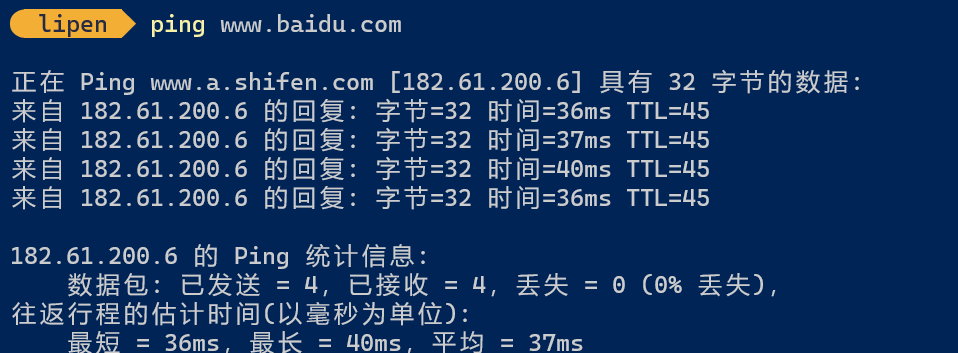
\includegraphics[width=0.8\textwidth]{images/01.png}
  \caption{使用\texttt{ping}命令发起\texttt{ICMP}请求}
\end{figure}

打开\texttt{Wireshark},在菜单栏的捕获\(\to \)选项中进行设置,选择已连接的以太网,设置捕获过滤器为\texttt{icmp},将混杂模式设为关闭,勾选\texttt{enable MAC name resolution}。然后开始捕获。

\begin{figure}[H]
  \centering
  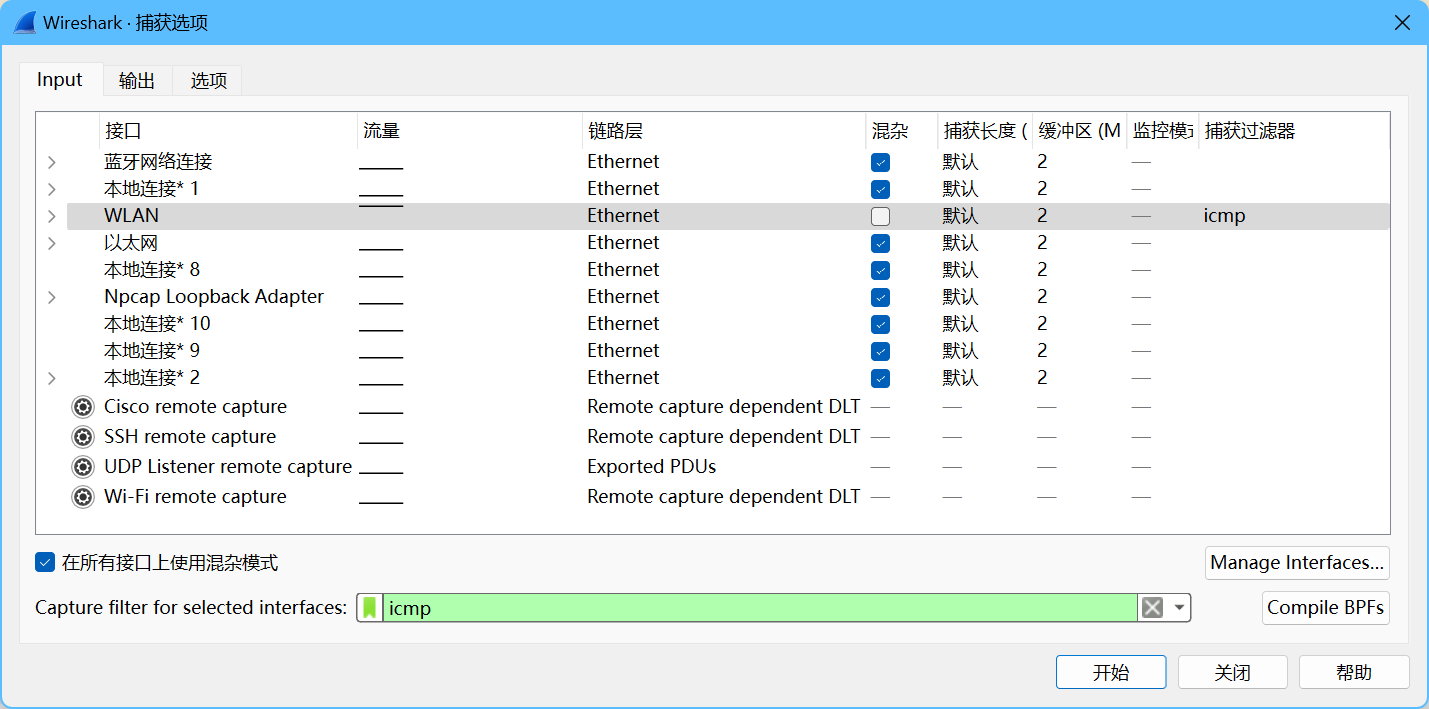
\includegraphics[width=0.8\textwidth]{images/02.png}
  \caption{设置\texttt{Wireshark}捕获过滤器}
\end{figure}

回到命令行,再次使用\texttt{ping}命令发起\texttt{ICMP}请求。

\begin{figure}[H]
  \centering
  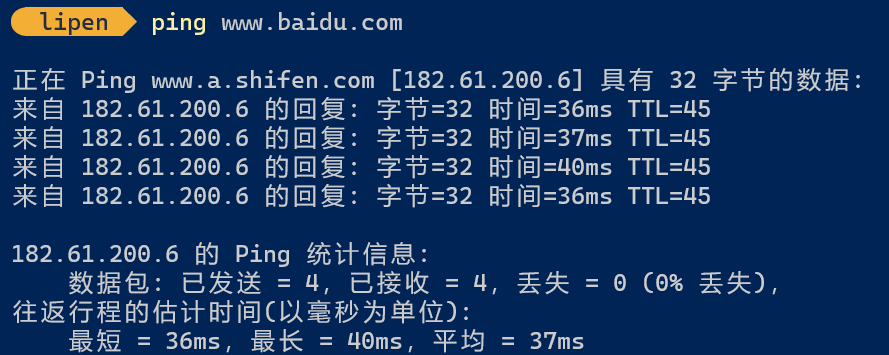
\includegraphics[width=0.8\textwidth]{images/03.png}
  \caption{再次使用\texttt{ping}命令发起\texttt{ICMP}请求}
\end{figure}

回到\texttt{Wireshark},停止捕获。捕获结果如下图所示:

\begin{figure}[H]
  \centering
  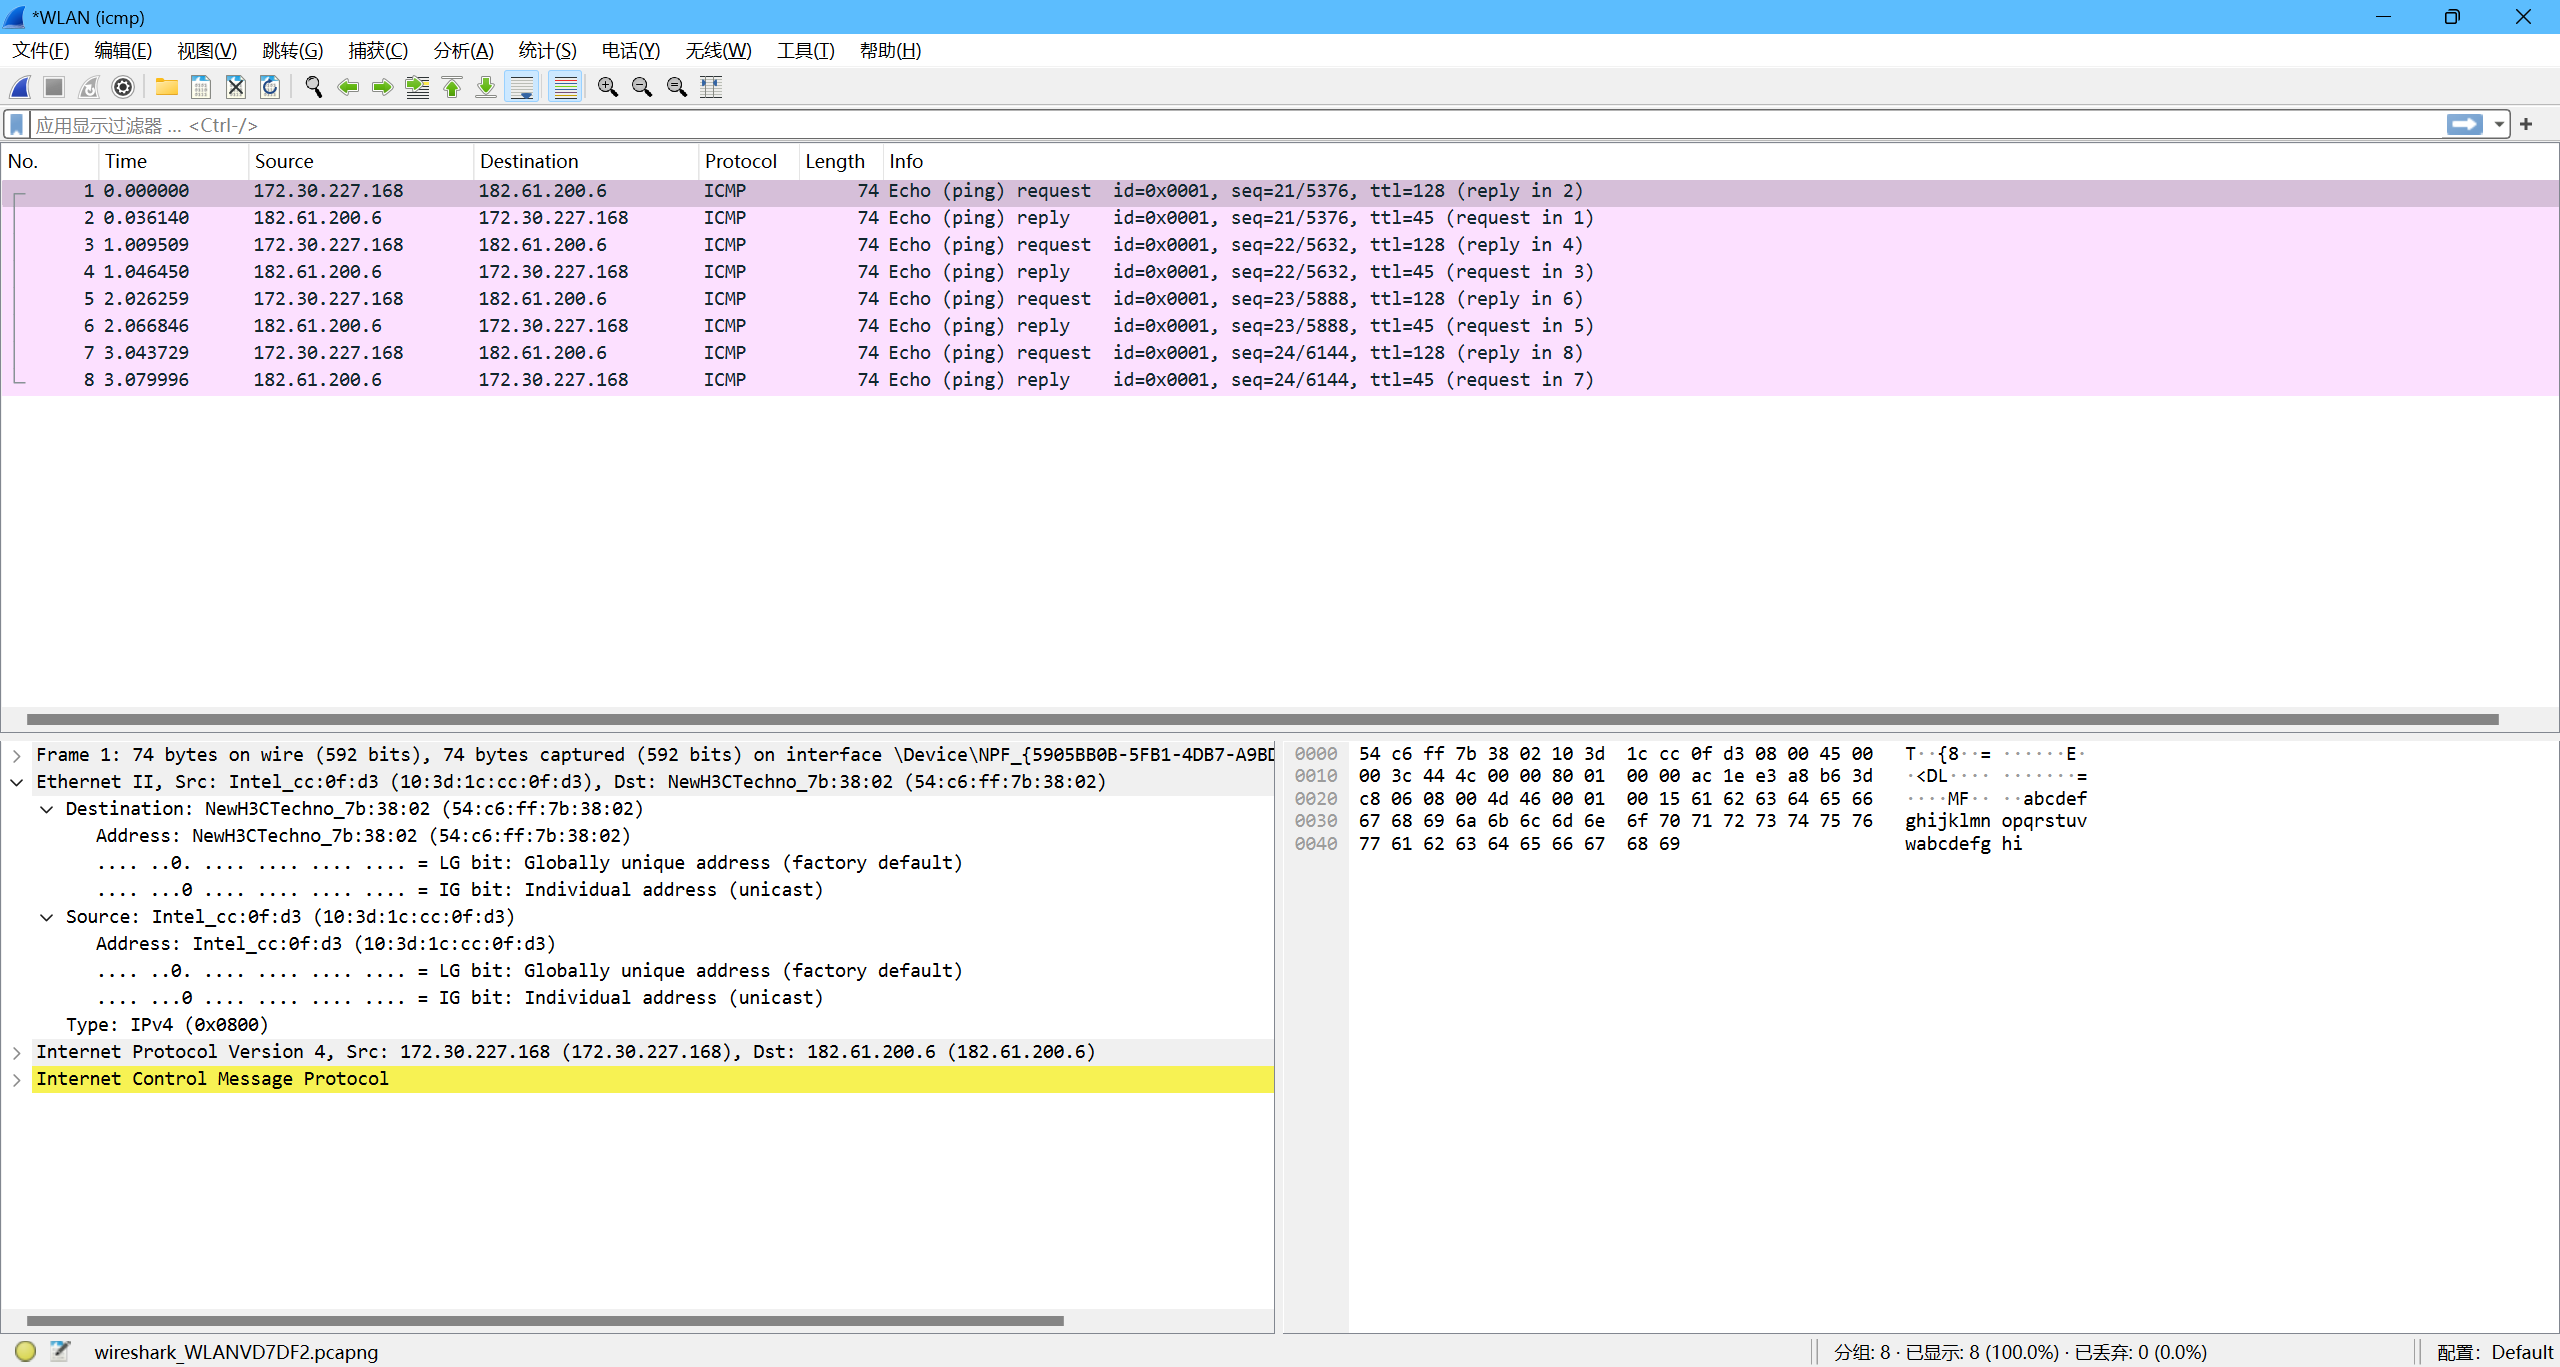
\includegraphics[width=0.8\textwidth]{images/04.png}
  \caption{捕获结果}
\end{figure}

\subsection{分析以太网的单播帧}

\textbf{问题:基于对以太网帧格式的理解,绘制ping消息的图形,该图形以字节为单位显示以太网报头字段的位置和大小。图形可以简单地将框架显示为一个细长的矩形。先出现在包中的是最左边的字段,会先通过网络发送。在此图中,显示以太网报头和以太网负载的范围。最后添加一个虚线框来表示4字节校验和。}

点击捕获到的数据包,选择\texttt{Ethernet II},可以看到\texttt{以太网}的帧结构如下图所示:

\begin{figure}[H]
  \centering
  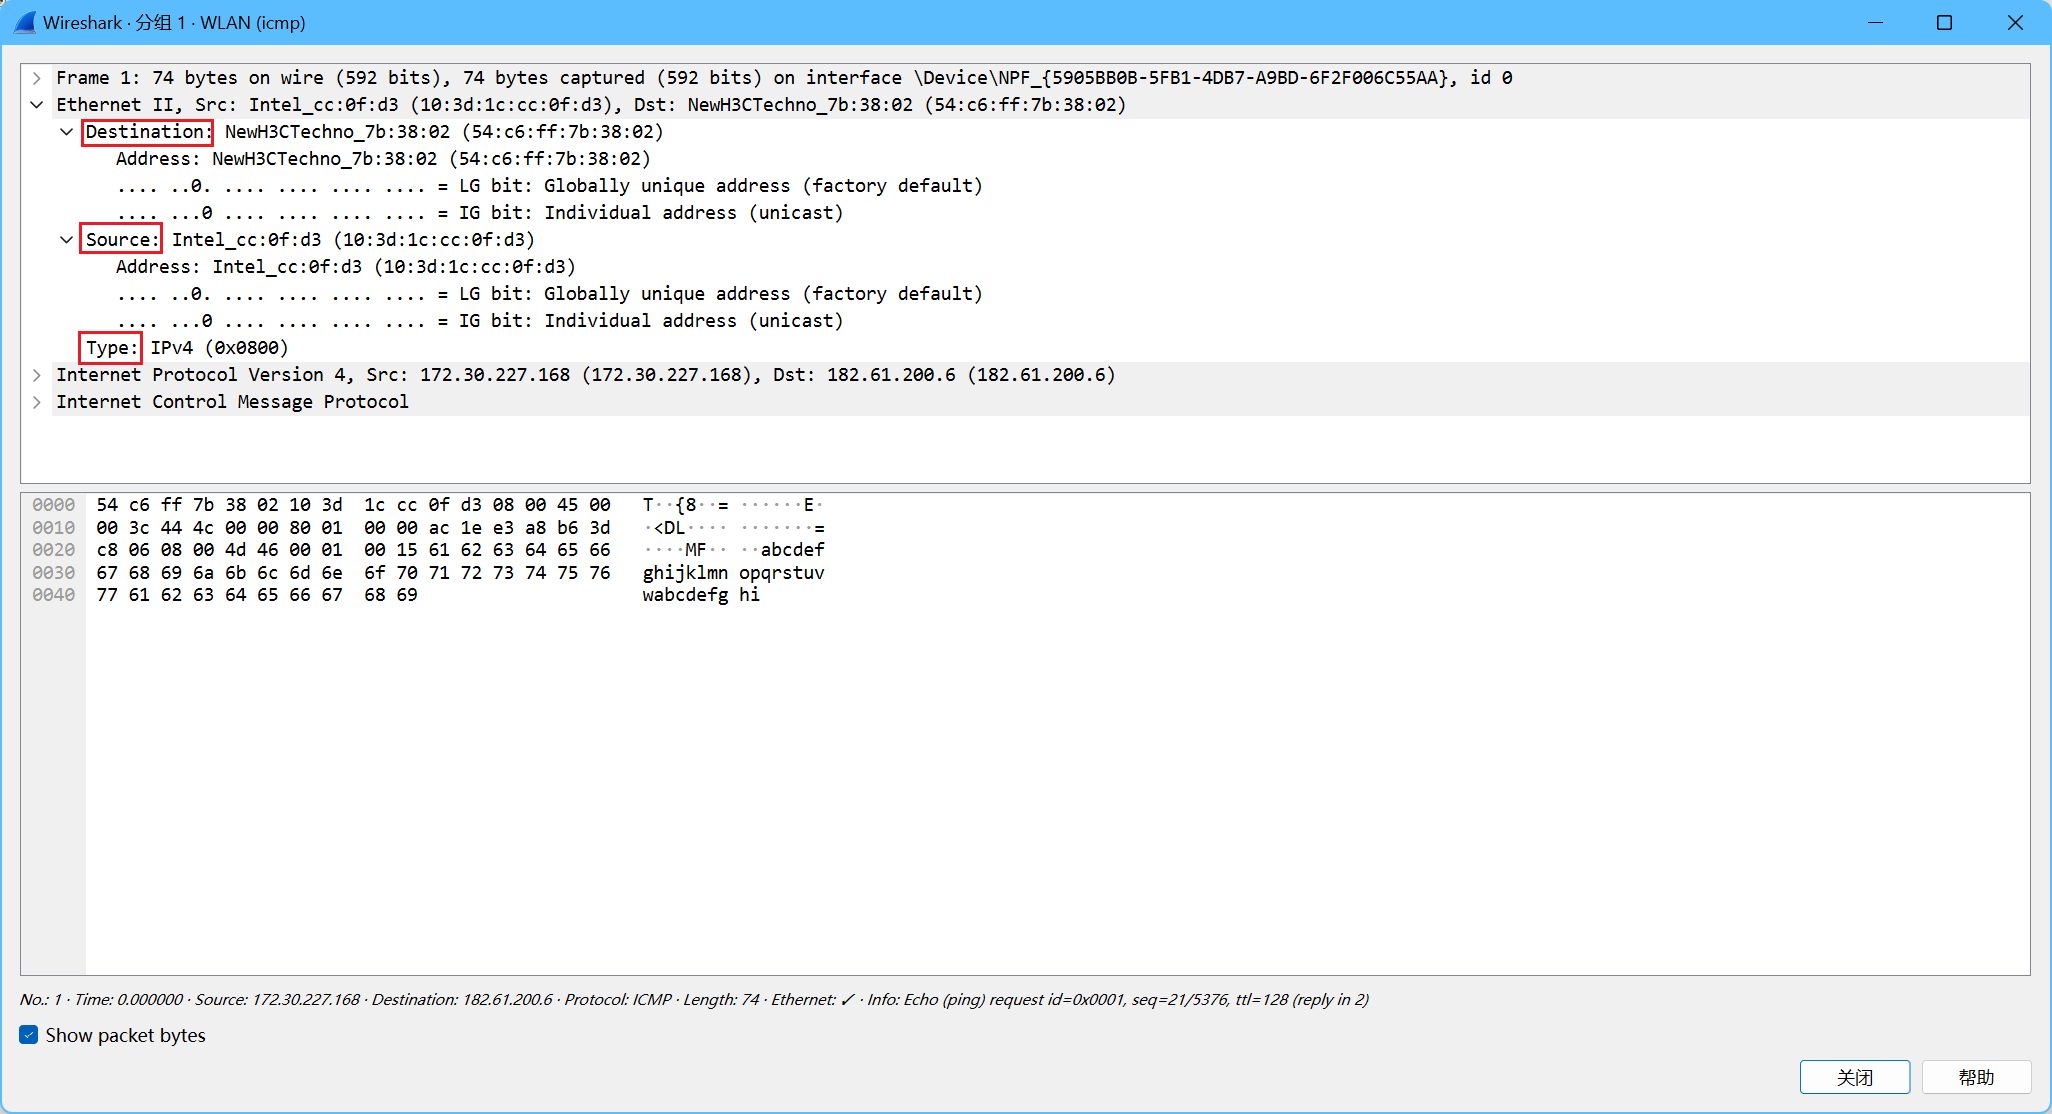
\includegraphics[width=0.8\textwidth]{images/05.png}
  \caption{\texttt{以太网}的帧结构}
\end{figure}

可以看到\texttt{以太网}头部包括了\texttt{目的地址(Destination)}、\texttt{源地址(Source)}和\texttt{类型(Type)}三部分。其中\texttt{目的地址}和\texttt{源地址}都是\texttt{6}个字节,\texttt{类型}是\texttt{2}个字节。

\begin{figure}[H]
  \centering
  \begin{minipage}[b]{0.42\textwidth}
    \centering
    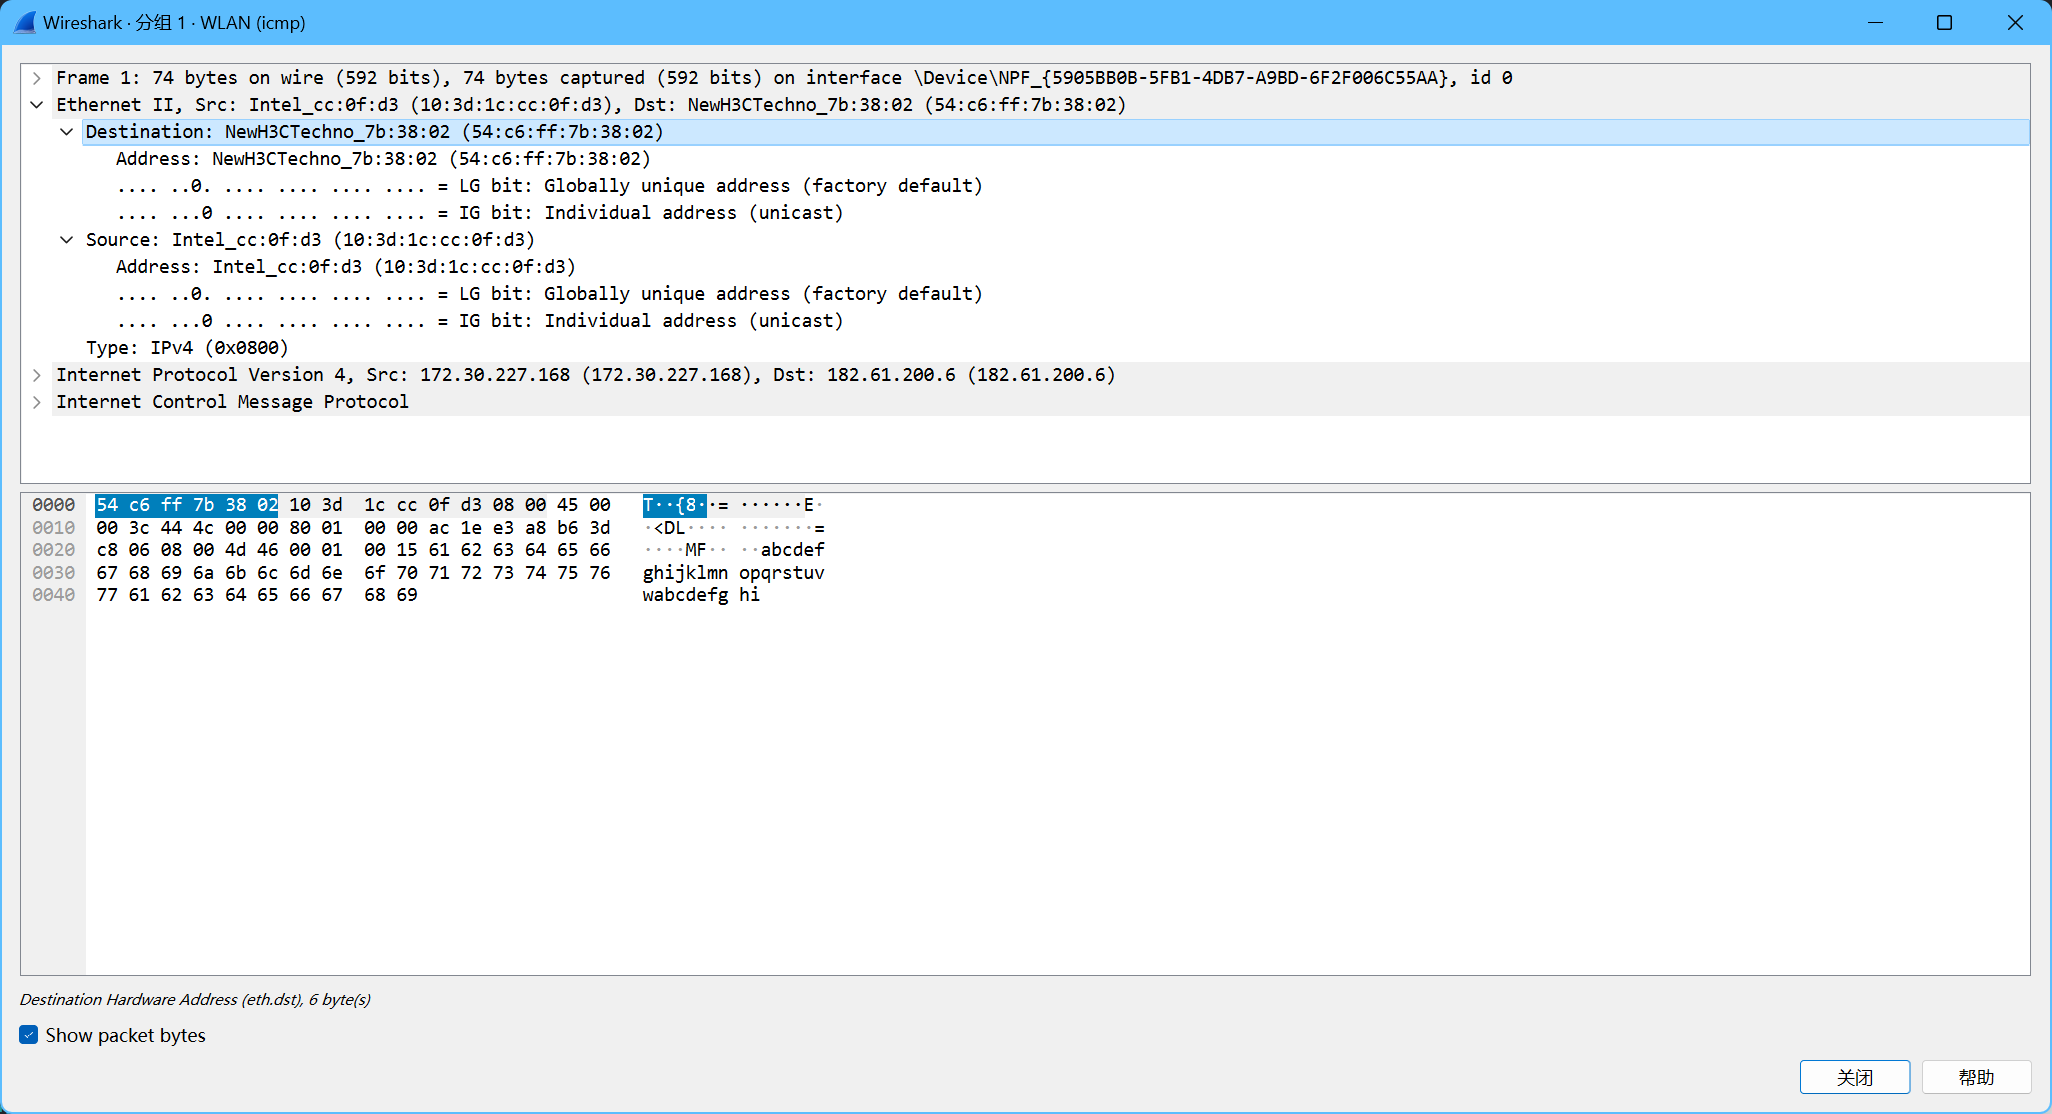
\includegraphics[width=\textwidth]{images/06.png}
    \caption{\texttt{Destination}}
  \end{minipage}
  \hfill
  \begin{minipage}[b]{0.42\textwidth}
    \centering
    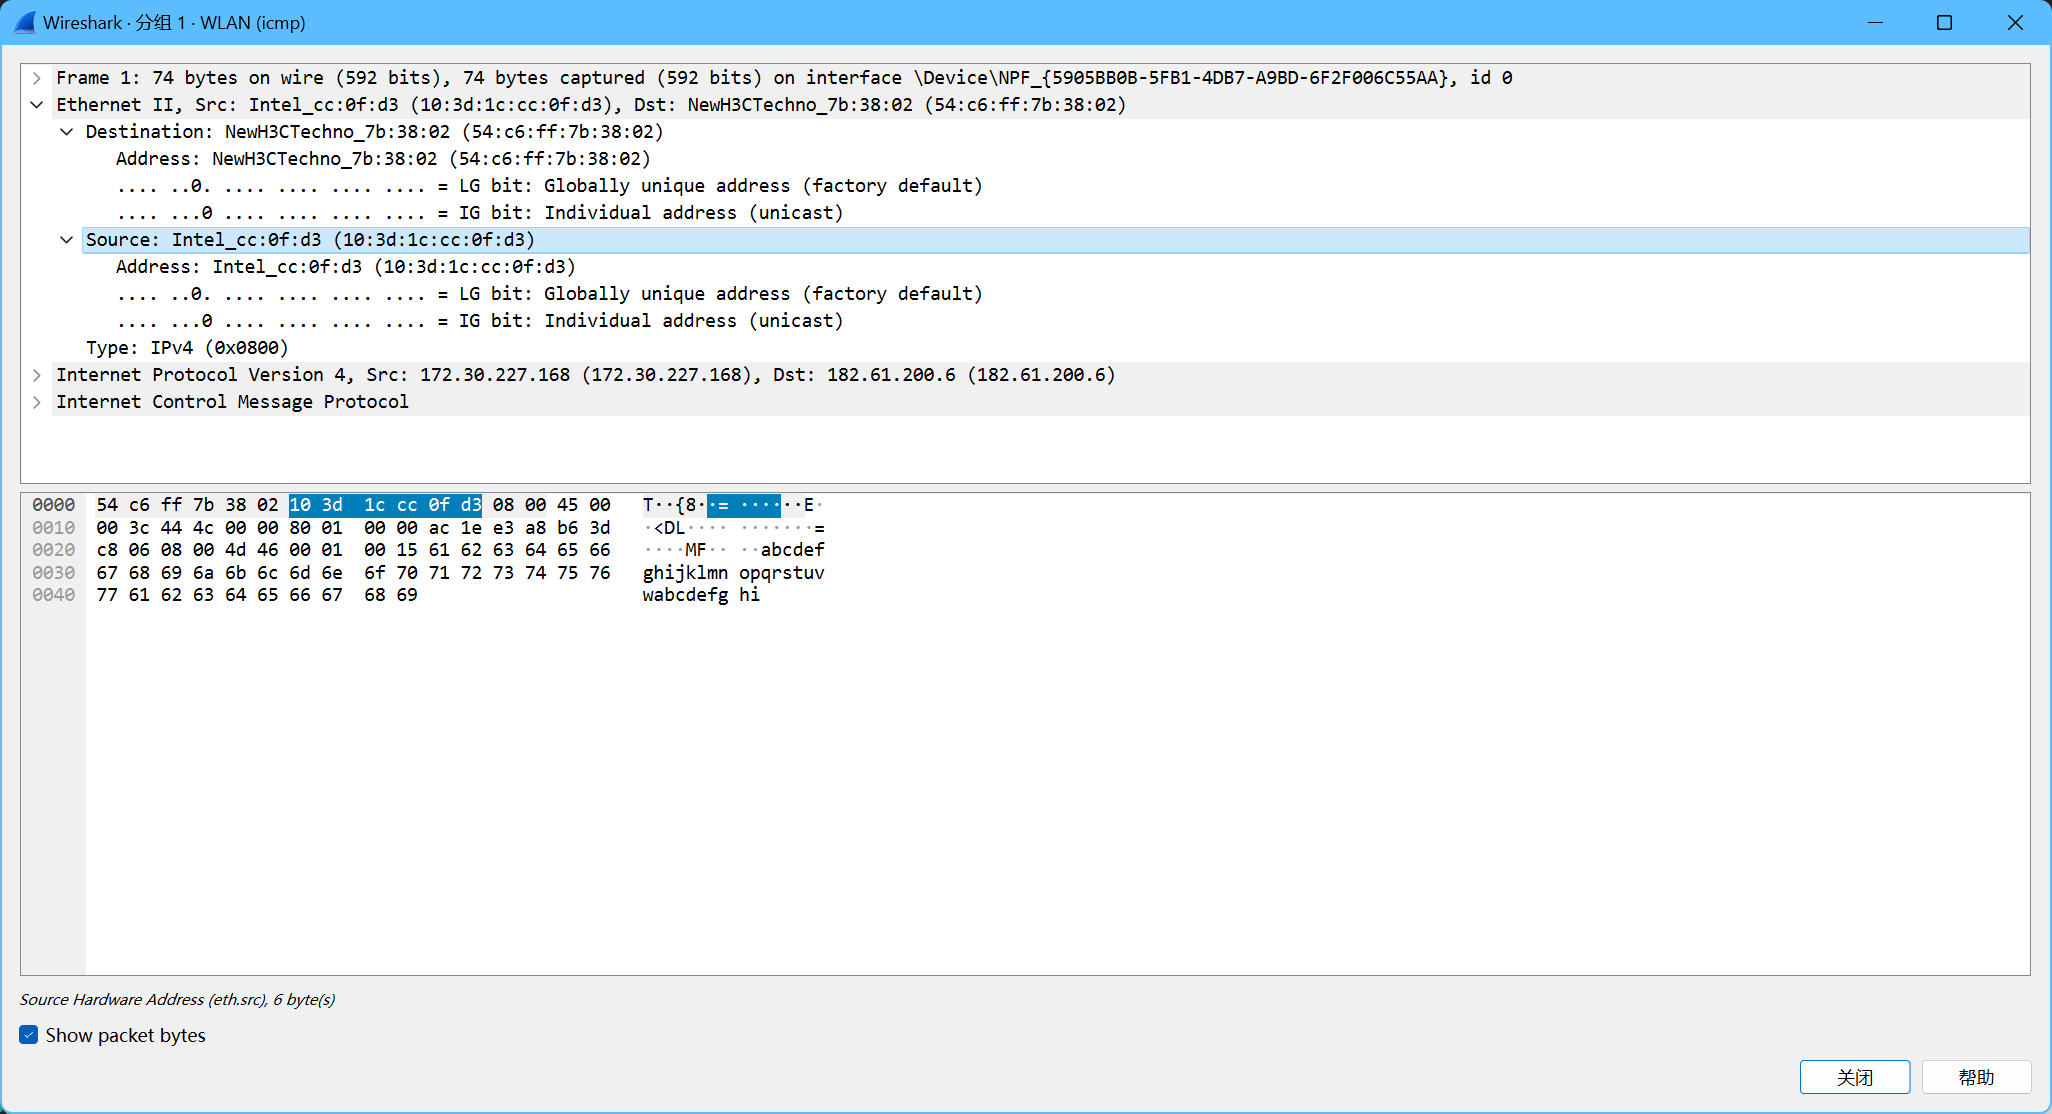
\includegraphics[width=\textwidth]{images/07.png}
    \caption{\texttt{Source}}
  \end{minipage}
\end{figure}

\begin{figure}[H]
  \centering
  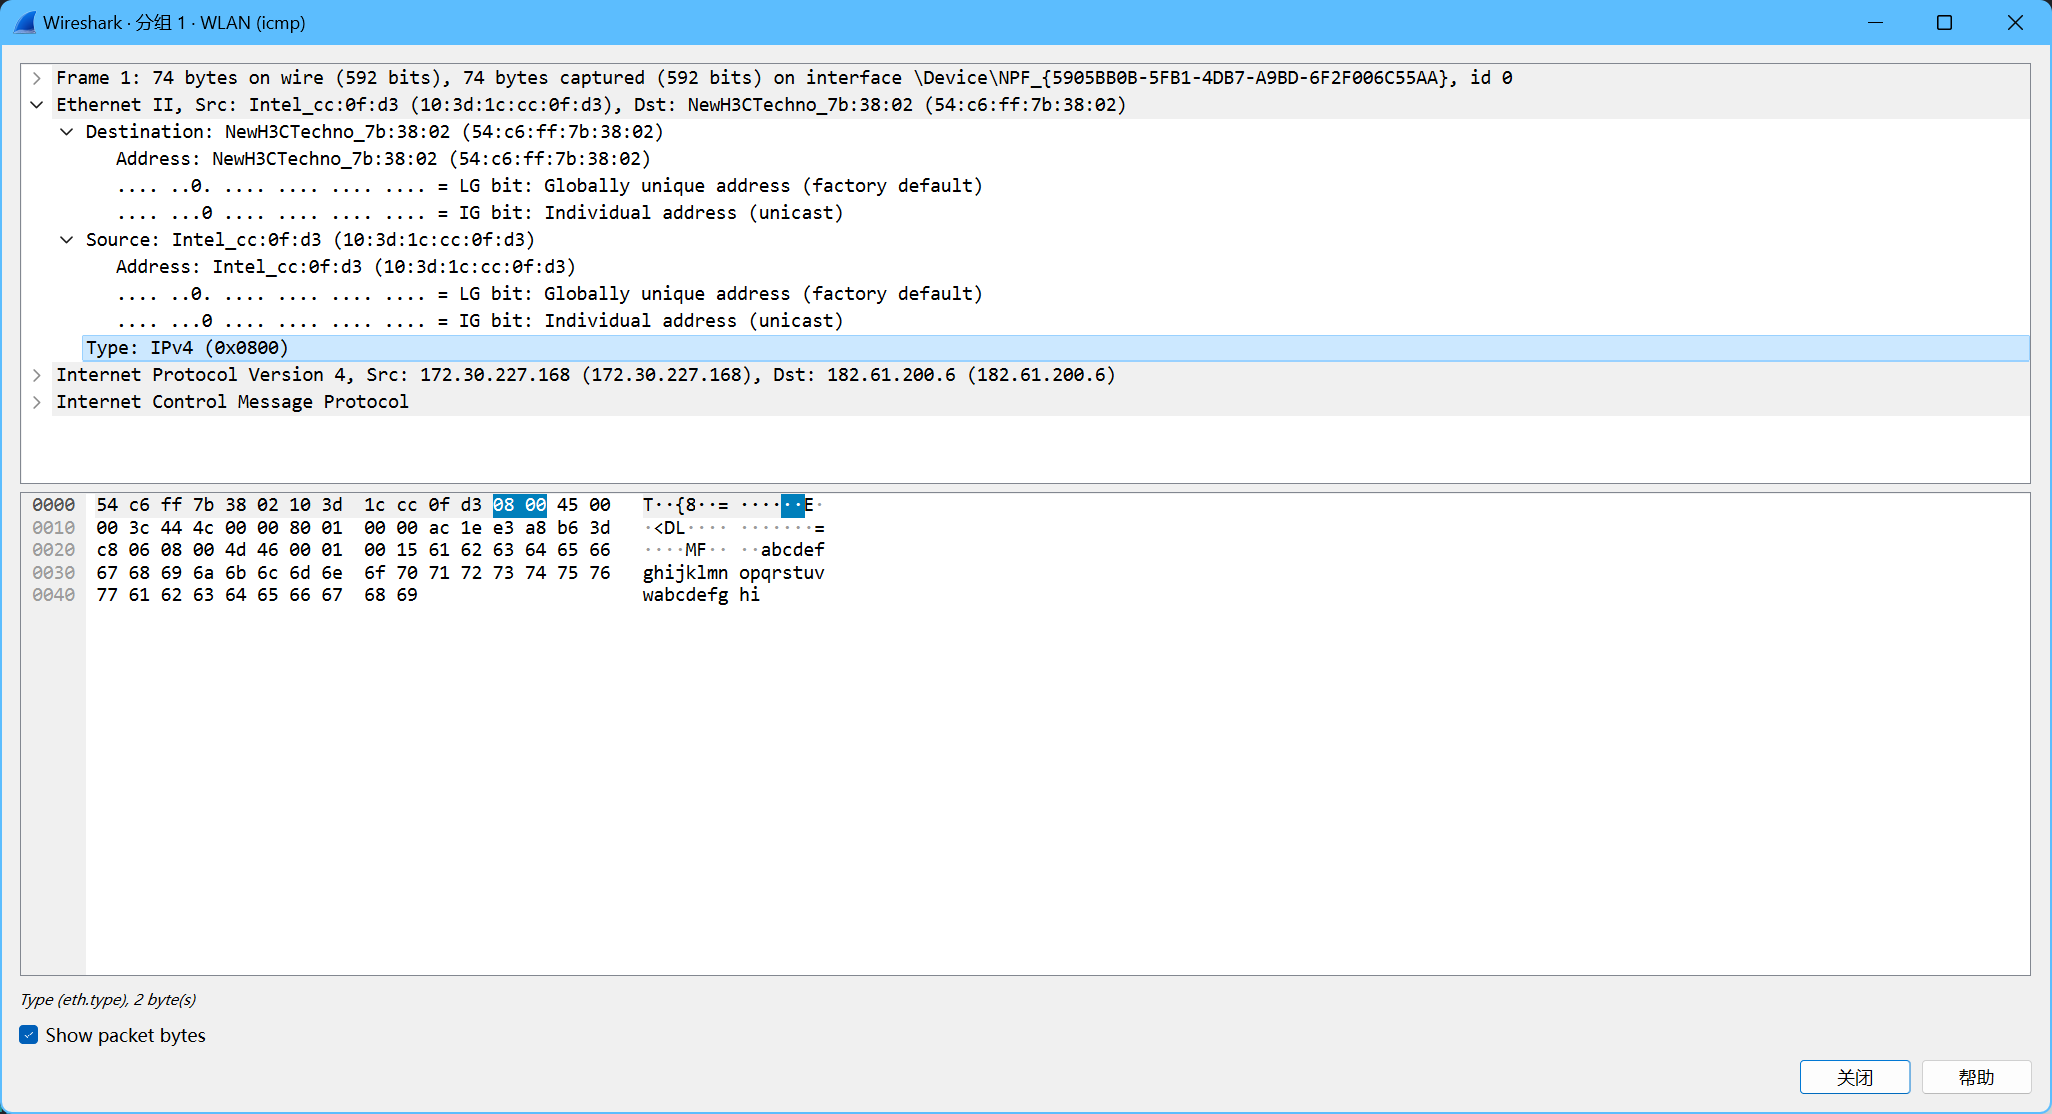
\includegraphics[width=0.42\textwidth]{images/08.png}
  \caption{\texttt{Type}}
\end{figure}

画出的帧结构如下图所示:

\begin{figure}[H]
  \centering
  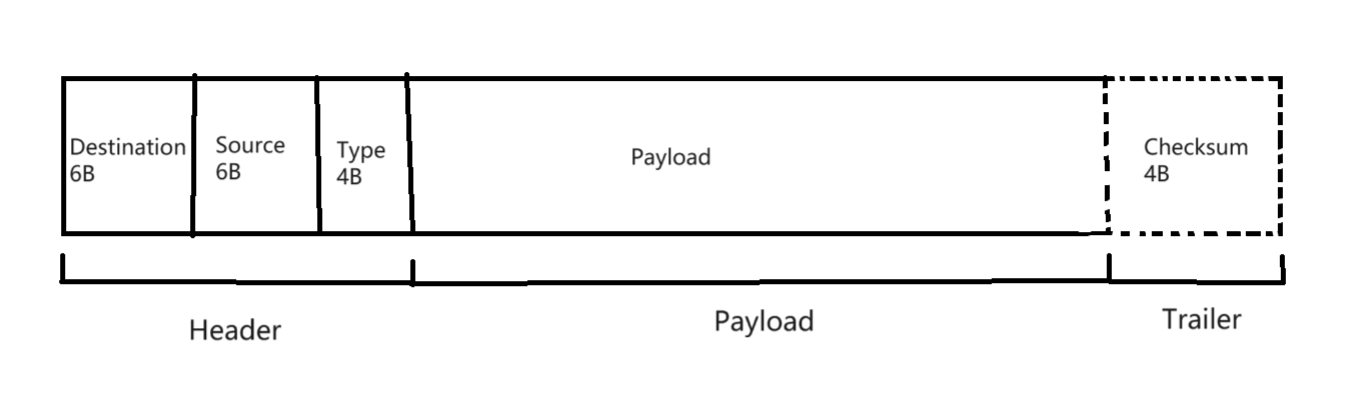
\includegraphics[width=0.8\textwidth]{images/09.png}
  \caption{\texttt{以太网}帧结构}
\end{figure}

\subsection{分析以太网的地址范围}

\textbf{画一个图,显示你的电脑,路由器和远程服务器的相对位置。标记你的电脑和路由器的以太网地址。标记你的计算机和远程服务器的IP地址。}

根据上面分析得到的\texttt{以太网}帧结构,我们可以得知本机\texttt{MAC}地址为\texttt{10:3d:1c:cc:0f:d3},\texttt{IP}地址为\\\texttt{172.30.227.168},路由器\texttt{MAC}地址为\texttt{54:c6:ff:7b:38:02},目标\texttt{IP}地址为\texttt{182.61.200.6}。

可以作出如下的关系图:

\begin{figure}[H]
  \centering
  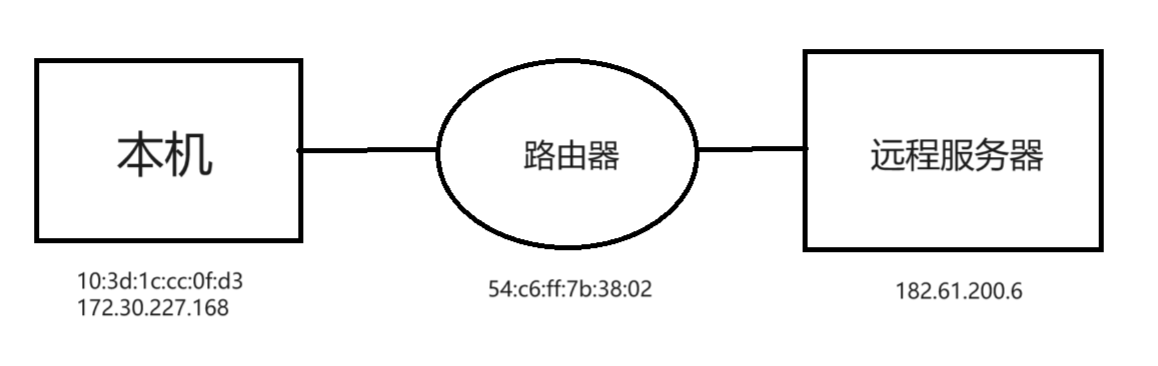
\includegraphics[width=0.8\textwidth]{images/10.png}
  \caption{\texttt{以太网}地址范围关系图}
\end{figure}

\subsection{分析以太网的广播帧或多播帧}

启动\texttt{Wireshark},在菜单栏的捕获\(\to \)选项中进行设置,选择已连接的以太网,设置捕获过滤器为\texttt{ether multicast},捕获\texttt{以太网}的广播帧。

\begin{figure}[H]
  \centering
  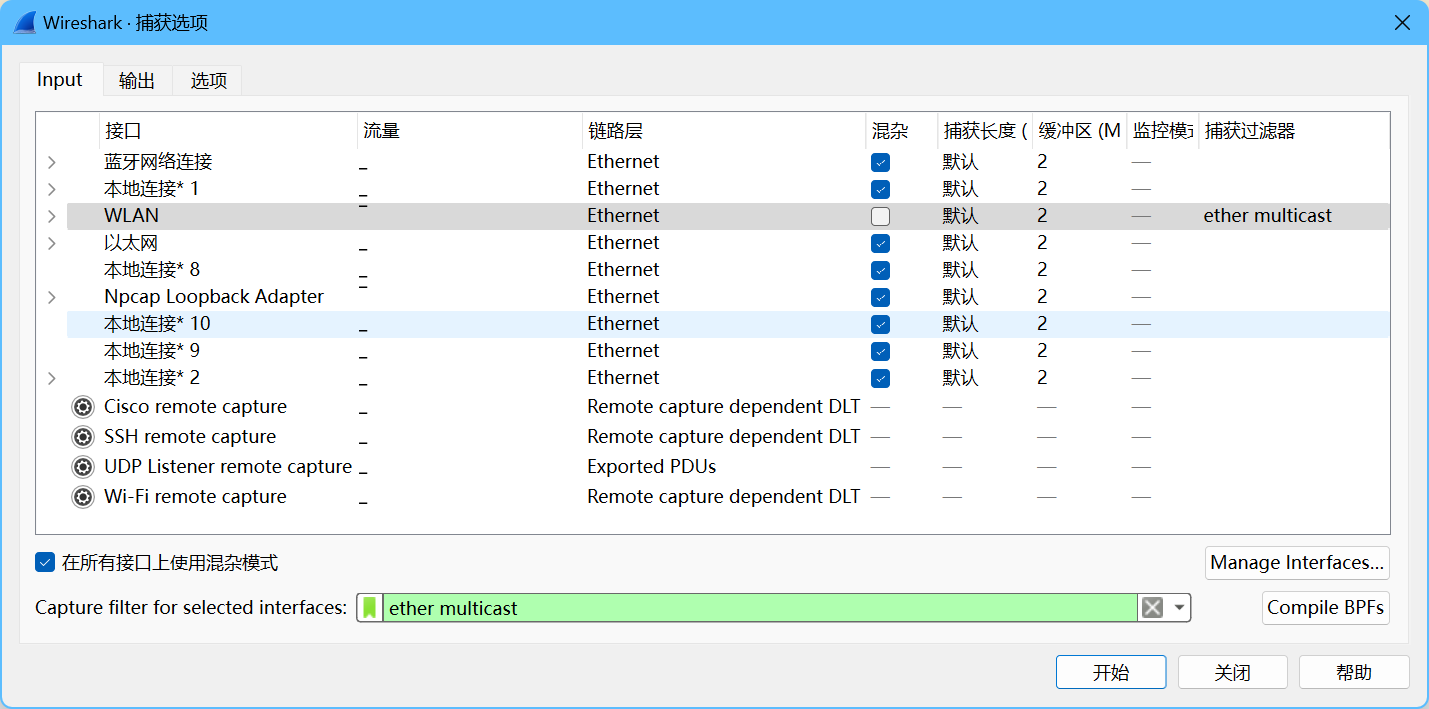
\includegraphics[width=0.6\textwidth]{images/11.png}
  \caption{设置\texttt{Wireshark}捕获过滤器}
\end{figure}

经过一段时间的捕获,捕获结果如下图所示:

\begin{figure}[H]
  \centering
  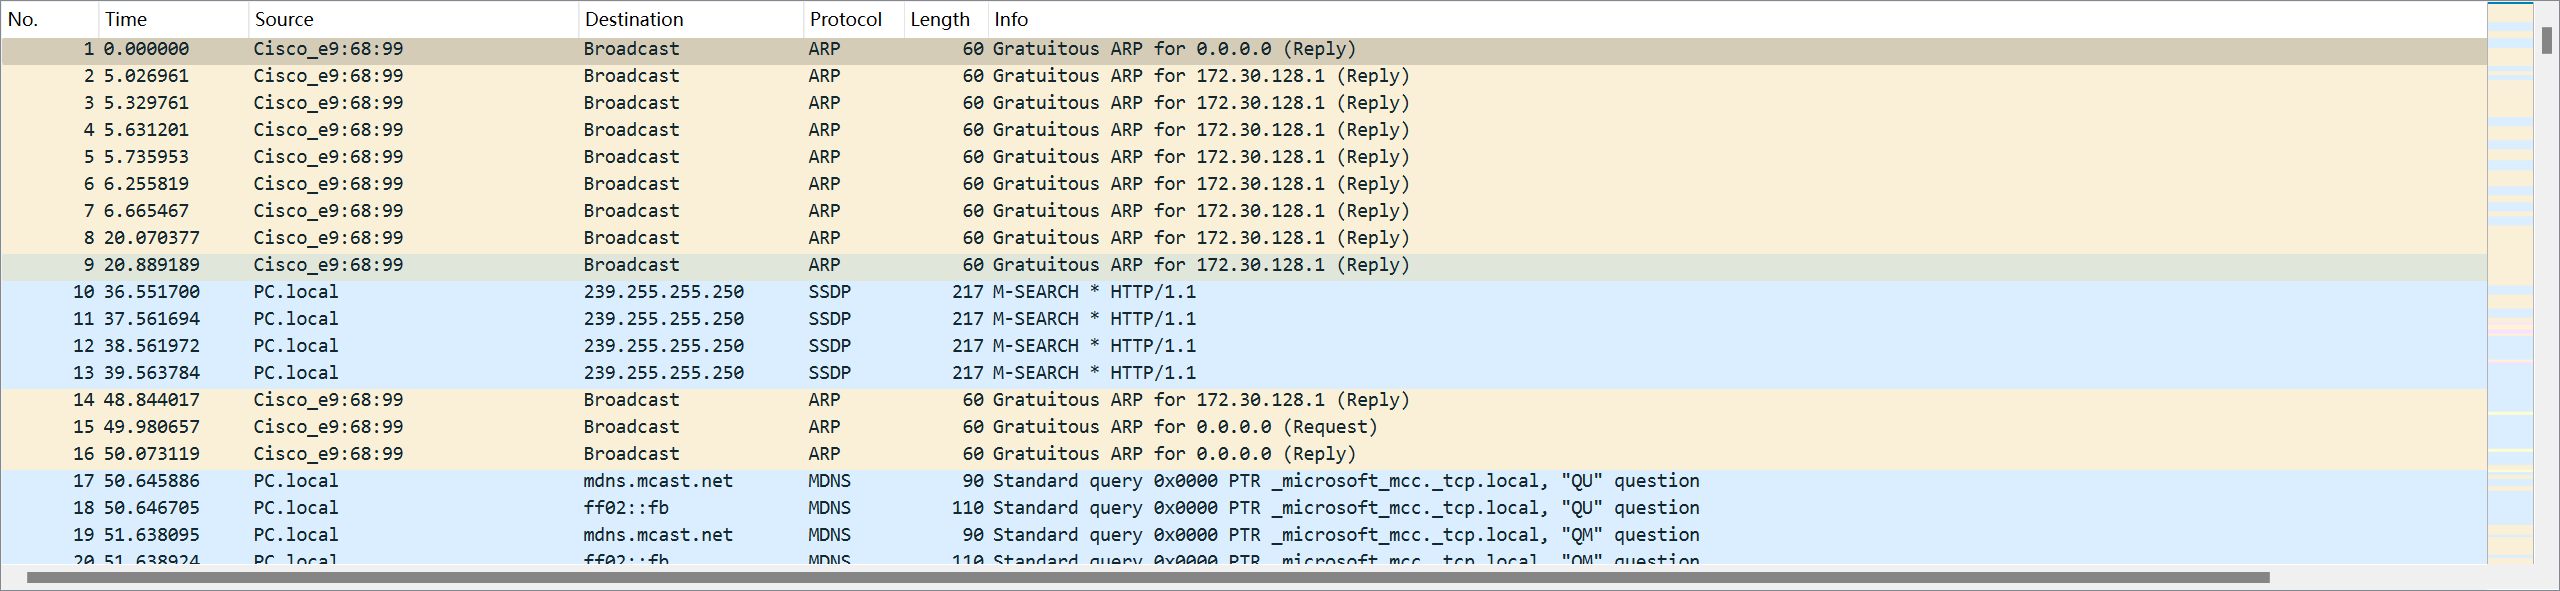
\includegraphics[width=0.8\textwidth]{images/12.png}
  \caption{捕获结果}
\end{figure}

选择其中的一个广播帧数据包,如下图所示:

\begin{figure}[H]
  \centering
  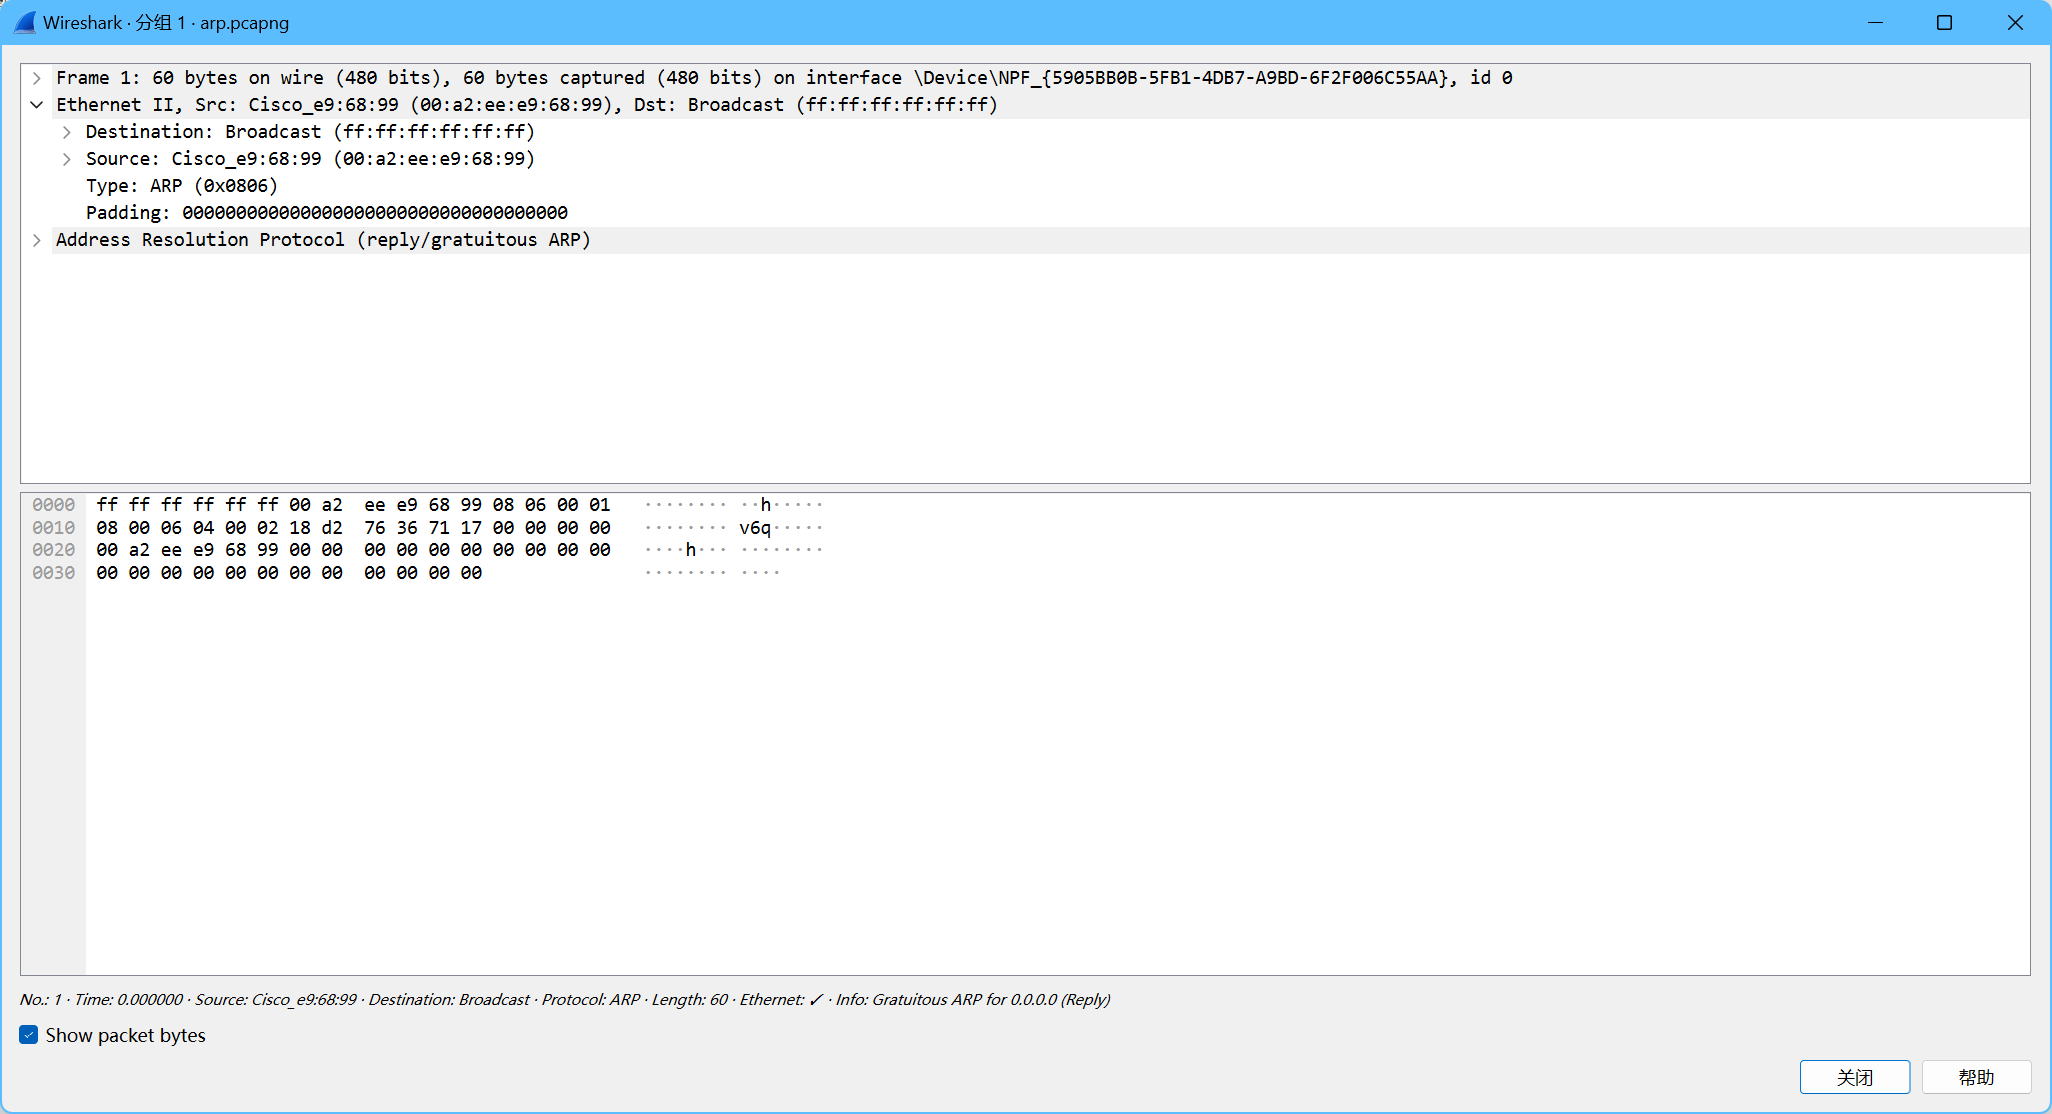
\includegraphics[width=0.75\textwidth]{images/13.png}
  \caption{广播帧数据包}
\end{figure}

\textbf{问题:}

\begin{enumerate}[noitemsep]
  \item \textbf{以太网广播帧的地址是什么,以标准的形式写在Wireshark上显示?}

        可以看出,广播帧的地址为\texttt{ff:ff:ff:ff:ff:ff}。

        \begin{figure}[H]
          \centering
          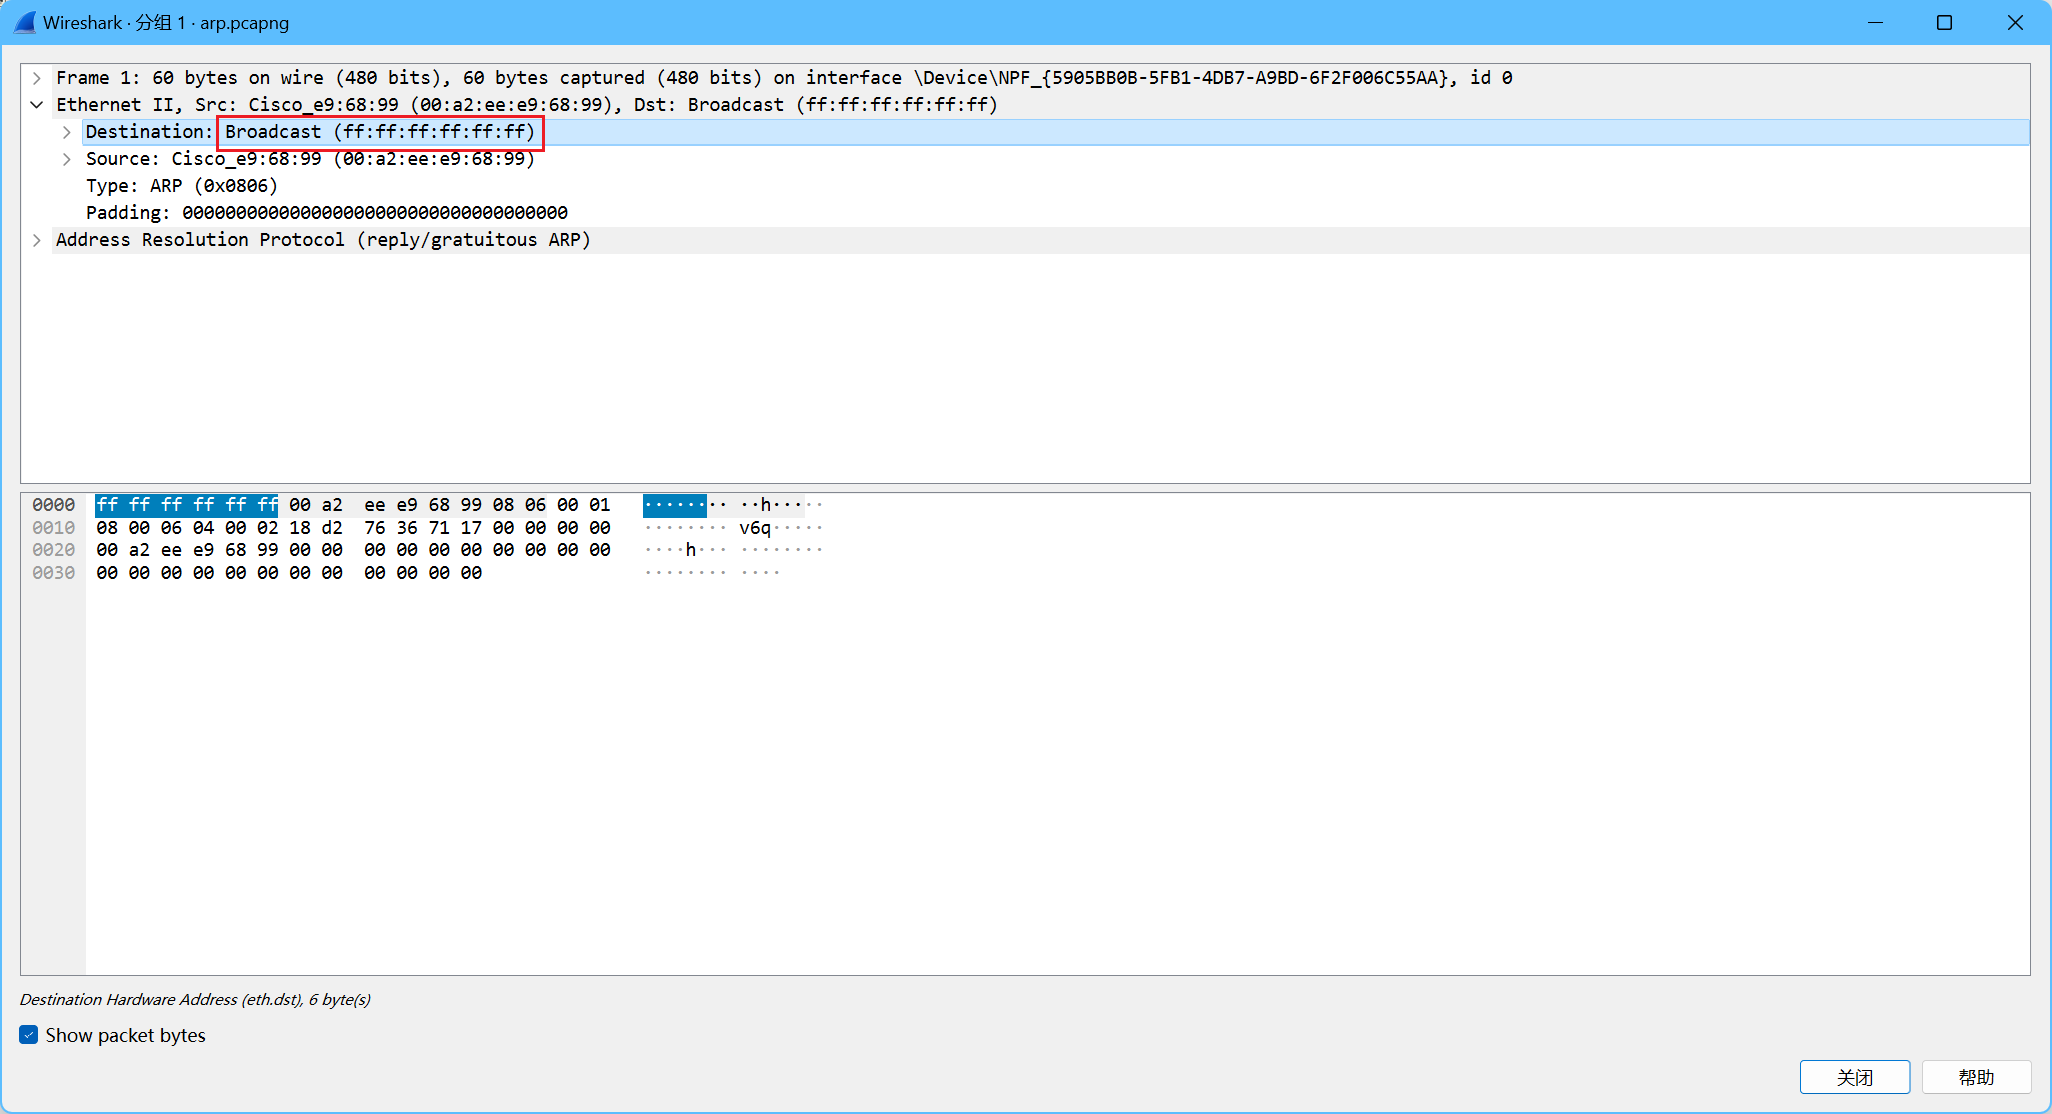
\includegraphics[width=0.75\textwidth]{images/14.png}
          \caption{广播帧地址}
        \end{figure}

  \item \textbf{哪几个比特位的以太网地址是用来确定是单播或多播/广播?}

        对比单播帧和广播帧,可以看出,\texttt{以太网}地址的第一个字节的最后一位(即第八位)为\texttt{1},所以可以确定是多播/广播。

        \begin{figure}[H]
          \centering
          \begin{minipage}[b]{0.48\textwidth}
            \centering
            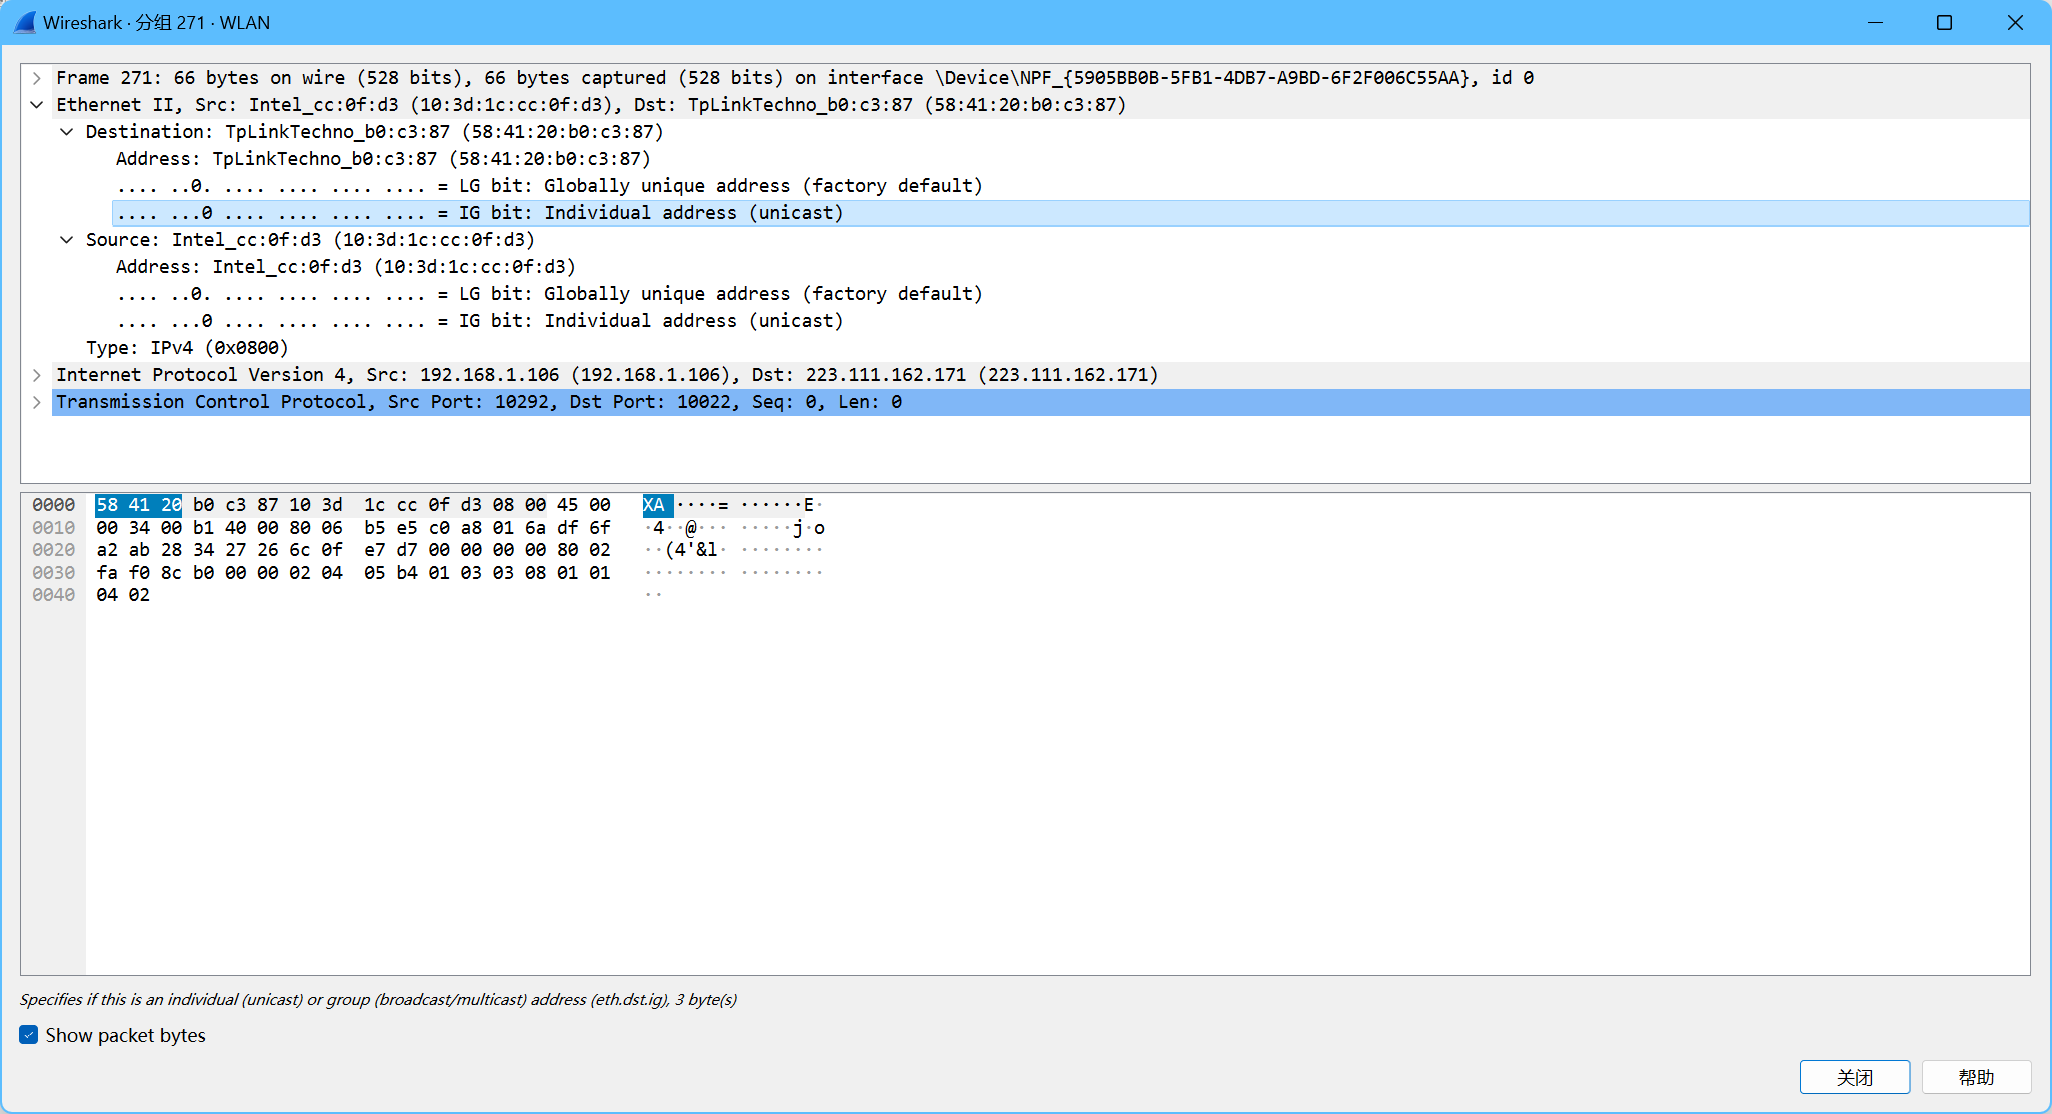
\includegraphics[width=\textwidth]{images/16.png}
            \caption{单播帧}
          \end{minipage}
          \hfill
          \begin{minipage}[b]{0.48\textwidth}
            \centering
            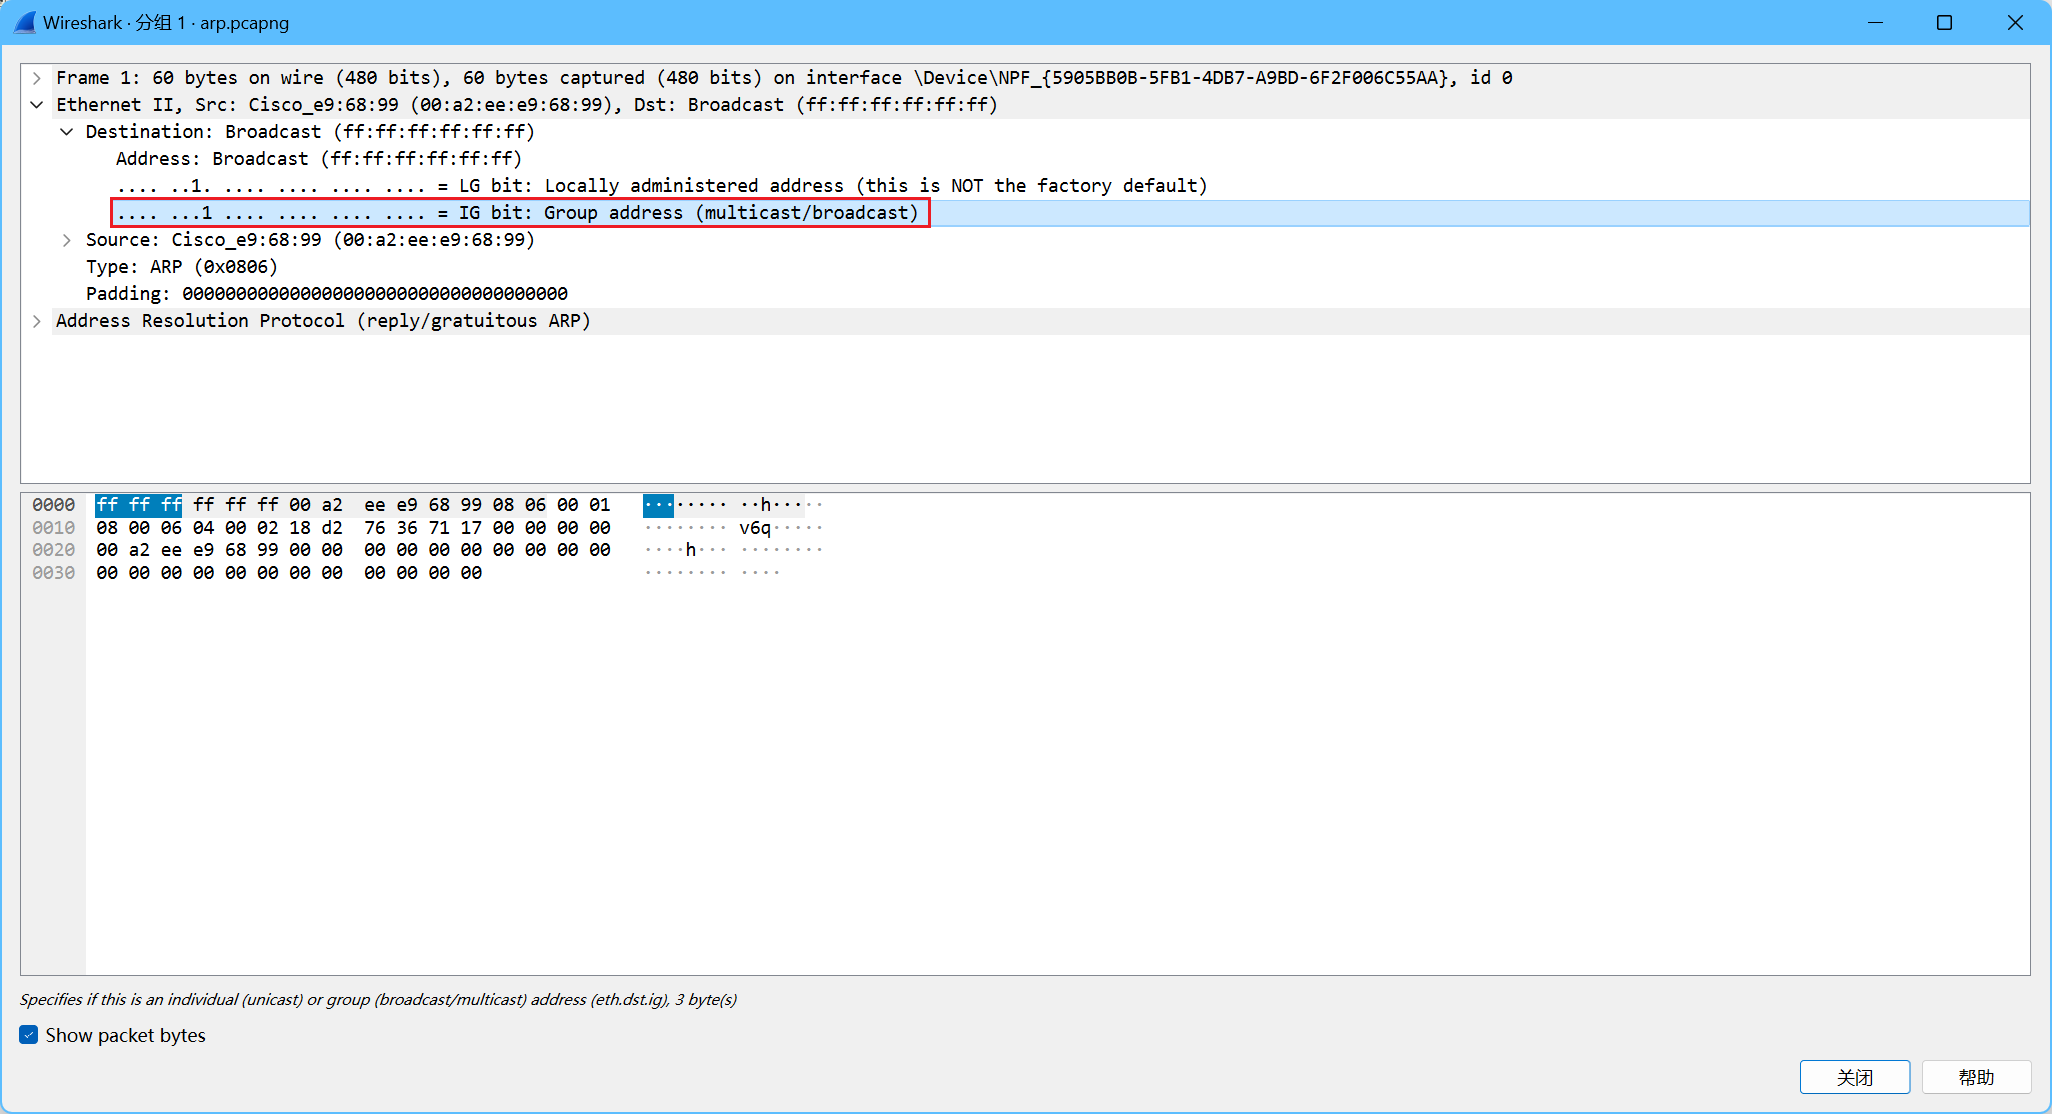
\includegraphics[width=\textwidth]{images/15.png}
            \caption{广播帧}
          \end{minipage}
        \end{figure}
\end{enumerate}

\subsection{问题讨论}

设置捕获过滤器为\texttt{llc},捕获\texttt{以太网}的帧,如下图所示:

\begin{figure}[H]
  \centering
  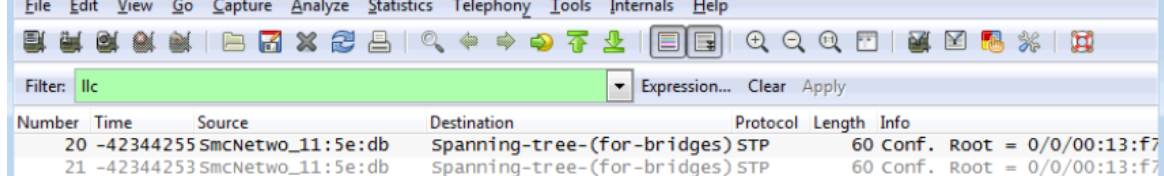
\includegraphics[width=0.75\textwidth]{images/17.png}
  \caption{捕获\texttt{IEEE 802.3 以太网}的帧}
\end{figure}

\begin{enumerate}[noitemsep]
  \item \textbf{与DIX以太网报头相比,IEEE 802.3和LLC组合报头有多长?
  您可以使用Wireshark解决此问题。 请注意,Trailer / Padding和Checksum可能显示为标头的一部分,但它们位于帧的末尾。}
  

        \textbf{答:}DIX以太网头部长度为\texttt{14}字节,IEEE 802.3头部长度为\texttt{14}字节,LLC头部长度为\texttt{3}字节。如下图所示:

        \begin{figure}[H]
          \centering
          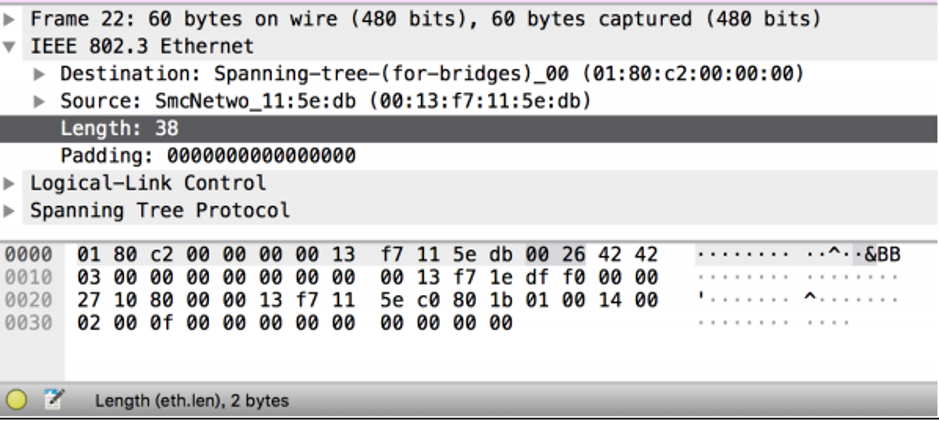
\includegraphics[width=0.75\textwidth]{images/18.png}
          \caption{\texttt{IEEE 802.3 以太网}头部}
        \end{figure}

  \item \textbf{接收方计算机如何知道该帧是DIX以太网还是IEEE 802.3? 提示:您可能需要同时使用Wireshark查看数据包示例并查找相关文献。}

        \textbf{答:}根据\texttt{Type/Length}字段,如果该字段的值小于或等于\texttt{1500},则表示\texttt{Length},为IEEE 802.3,否则表示\texttt{Type},为DIX以太网。

        \begin{figure}[H]
          \centering
          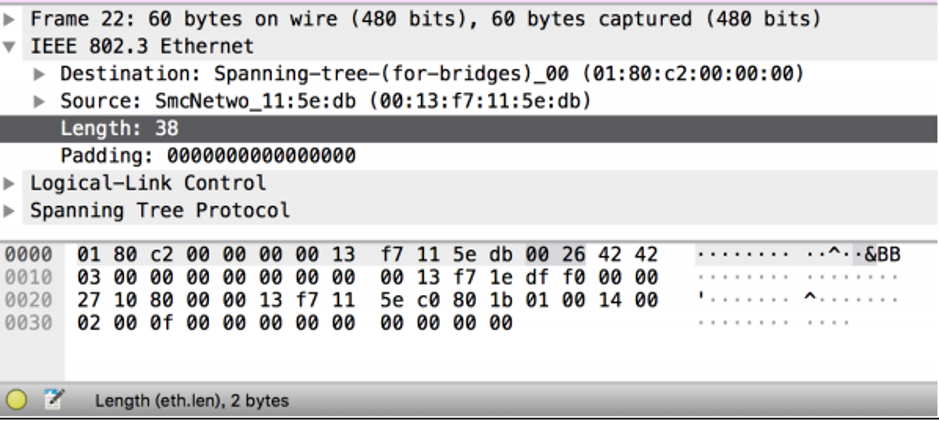
\includegraphics[width=0.7\textwidth]{images/18.png}
          \caption{\texttt{Length}字段}
        \end{figure}

  \item \textbf{如果IEEE 802.3没有类型字段,那么如何确定下一层? 使用Wireshark查找解复用键。}

        \textbf{答:}\texttt{LLC}头中的\texttt{DSAP}字段可以指示上层协议。例如,此处\texttt{DSAP}字段为\texttt{0x42},则表示上层协议为\texttt{STP}。

        \begin{figure}[H]
          \centering
          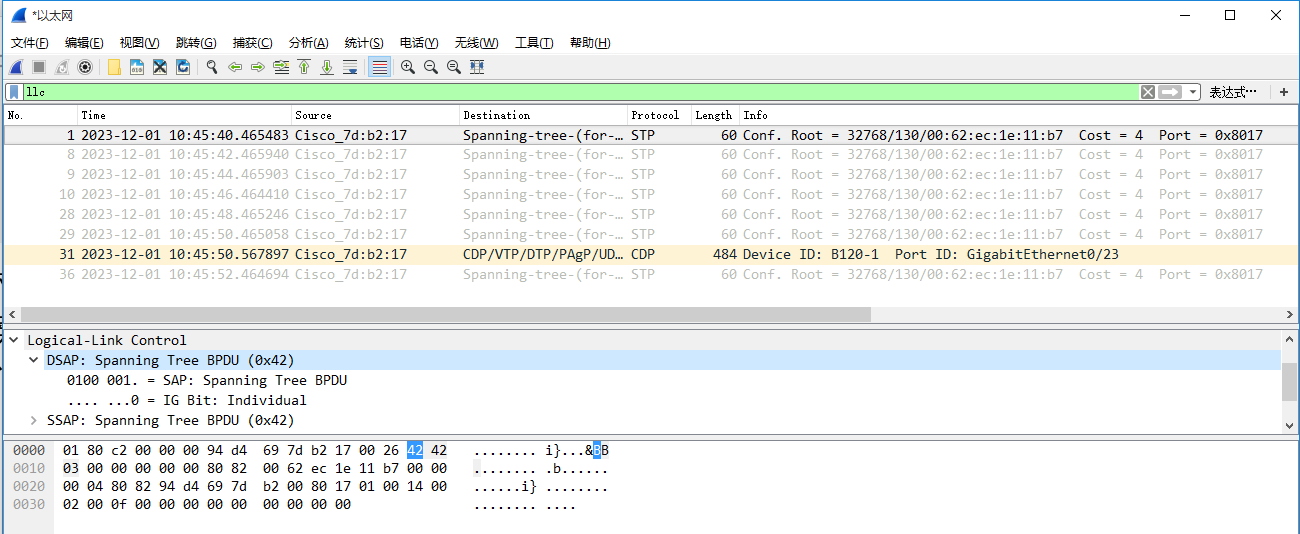
\includegraphics[width=0.75\textwidth]{images/19.png}
          \caption{\texttt{DSAP}字段}
        \end{figure}

\end{enumerate}


\section{实验结果总结}

通过本次实验,我学会了通过\texttt{Wireshark}获取\texttt{以太网}的帧,掌握了\texttt{以太网}帧的结构,分析了\texttt{以太网}地址范围,分析了\texttt{以太网}的广播帧。同时,我还了解到了\texttt{DIX 以太网}和\texttt{IEEE 802.3 以太网}的区别。

\section{附录}

无

\end{document}